\section{Systematic Review}
\label{sec:systematic-review}

What distinguishes this paper among others — as we mentioned — we do recognize that the majority of recruiters do not have skills that could examine the technicality of a candidate. For example in the \emph{"Mining the Technical Roles of GitHub Users"} the survey was conducted among recruiters from StackOverflow website \footnote{StackOverflow Website URL: \url{https://stackoverflow.com/}} - which is primarily used by developers for the purposes of collaboration \& knowledge sharing. Thus, it can be concluded that the surveyed sample was exceptional among the global population of recruiters as they have made extra efforts to create an account on IT-technical website and not only that - they were actively browsing it and even possibly creating extra content which made them visible and reachable by researchers. Based on the research we have conducted, there are only a few unfinished recommendation systems that use the user GitHub profile, but at the same time there is some research that focuses on mining data from the repositories.

\subsection{Research Questions}
Research questions presented below should explain to help understand the importance of creating such a tool and provide information about the functionalities which the potential end user might need (i.e. - recruiters, developers themselves). Furthermore, we also explore issues related to the recruitment itself, as well as the quality of repositories.

Hence, we defined four research questions.
\begin{itemize}
\item{\emph{RQ1: What are the most common skills the company is looking for among the candidates?}\\
  Our system needs to determine whether the developer is worthy of attention and if he should be considered further in the recruitment process. The answer to this question should explain what skills are considered important among companies. }
\item{\emph{RQ2: How a given repository makes a good impression?}\\
  One way of assessing developer expertise is to analyse his projects. Thus, we should determine which features of repositories are the most representative ones.} 
\item{\emph{RQ3: Is it possible to get a good enough information about the candidate's potential based on the GitHub profile?}\\
  This question should provide us with information whether the recommendation system based on repositories is worth devoting time.} 
\item{\emph{RQ4: Is GitHub repository used only for programming purposes?}\\
  It often happens that an item is used contrary to the original intention of the author. The same situation might occur with the repositories. There is no compulsion to prohibit the use of a repository for purposes other than development.}
\end{itemize}

\subsection{Currently Available Resources on the Subject}
We used search engines (Google Scholar and Scopus) to find proper resources and currently available papers on the subject that we are investigating in our paper, and then - to collect all relevant literature - we created a more specific search string which is given below\textit{ [ref: ~\ref{lst:search-string}]}.

% This is final v1.0.0 formatting - it looks better if the page breaks here // MJ %
\newpage

\begin{lstlisting}[language=Query, label={lst:search-string}, caption=Search String Query]
(
  skill AND
  repository AND
  ( github OR gitlab OR bitbucket )
) OR (
  recruitment OR hiring OR interview
) AND (
  programming AND purpose
) AND (
      "Computer Science"
) AND (
  mining AND software
)
\end{lstlisting}
Because of the enormous number of results in Scopus, we decided to add another limitation such as the required presence of ,,Software Engineering'' keyword and ,,2017-2021'' year constraint to narrow it down in time to only the most relevant studies.

This gave us a good amount of publications which needed to be further filtered by hand.  As shown on the literature identification figure~\textit{[ref: \ref{fig:literature-identification}]} search engines provided us with over two hundred publications. Unfortunately, many of them did not answer the previously established research questions and many of them were simply not in English nor Polish language so that we can understand them. After all, we have identified ten of the most important studies that are helpful in our topic.

\begin{figure}[htp]
\centering
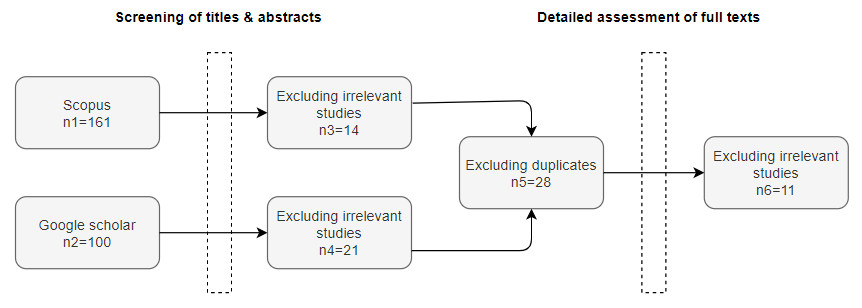
\includegraphics[width=\linewidth]{img/search_process_new.png}
\caption{Literature Identification}
\label{fig:literature-identification}
\end{figure}

% This is final v1.0.0 formatting - it looks better if the page breaks here // MJ %
\newpage

\subsection{Results Selection Process}
After running the search string query, we were presented with a large number of results. We have gone through the results list and discarded all duplicate entries and simultaneously discarded those papers whose titles or abstracts were not related to the topic of our research. Thus, we ended up with 28 papers which we further examined. Finally, we have chosen 10 papers which are closely related to the subject of this paper.
